\documentclass[preprint,3p,twocolumn,times,authoryear]{elsarticle}

\usepackage{wrapfig}
\usepackage[font=small]{caption}
\usepackage[hyperref,usenames,svgnames,dvipsnam]{xcolor}
\usepackage{subcaption}
\usepackage{amsmath}
\usepackage{mathtools}
\usepackage{bm}
\usepackage{breqn}
\usepackage{geometry}
%\usepackage{url}
\usepackage{booktabs}
\usepackage{multirow}
\usepackage{stfloats}
\usepackage{xfrac}
\usepackage{units}
\usepackage{tabularx}

\usepackage{siunitx}
\usepackage[colorlinks]{hyperref}

\bibliographystyle{model2-names}\biboptions{authoryear}

\journal{Icarus}

\begin{document}

\hypersetup{
     allcolors    = MidnightBlue
}

\begin{frontmatter}

\title{Numerically Modelling Ocean Dissipation in Icy Satellites: A Comparison of Linear and Quadratic Friction}

\author[label1]{Hamish C. F. C. Hay}
\author[label1]{Isamu Matsuyama}
\address[label1]{Lunar and Planetary Laboratory, University of Arizona, Tucson, AZ 85719, United States}

\begin{abstract}

\noindent Abstract

\end{abstract}
\end{frontmatter}

\newpage
\section{Introduction}

\hbadness=10000
\vbadness=10000

The primary source of heat generation in the outer Solar System icy satellites is energy lost via tidal dissipation. A result of this heating is the formation and potentially long term stable existence of global subsurface oceans, as has already been confirmed in several of the icy satellites. Europa has been shown to have an induced magnetic field consistent with a global layer of salty, liquid water beneath its surface \citep{zimmer2000subsurface, kivelson2000galileo, hand2007empirical}. This is also the case with Ganymede and Callisto, although these liquid oceans are likely to exist at least a few hundred kilometers beneath the surface \citep{zimmer2000subsurface, kivelson2000galileo}. Saturn's largest moon, Titan, has been interpreted to have a conductive liquid layer beneath its surface due a Schumann-like resonance \citep{beghin2010titan}, and this is supported by measurements of its mean moment of inertia \citep{bills2011rotational}. Enceladus also shows signs of a liquid ocean confined to its southern hemisphere. Evidence for this includes emission and composition of cryovolcanic plumes from a series of tidally induced shear faults over its south pole \citep{hansen2011composition}, as well as a detected negative mass anomaly consistent with a subsurface ocean \citep{iess2014gravity}. 

Despite this overwhelming evidence and abundance of subsurface oceans in the icy satellites, previous tidal dissipation studies have not been able to account for the energy needed to sustain these oceans over time. Many of these studies have primarily focused on tidal dissipation in the solid regions of the satellite \citep[e.g.,][]{moore2000tidal, roberts2008tidal, beuthe2013spatial}, ignoring the effects of a subsurface ocean. This is somewhat surprising as ocean dissipation is expected to dominate energy loss in the system, as is the case for Earth.

Other previous works on tidal dissipation within the icy satellites have considered a rather idealised case with only a global surface ocean, completely ignoring the effects of a solid lid \citep{sagan1982tide, sears1995tidal, sohl1995tidal, tyler2008strong, matsuyama2014tidal}. By assuming that there is no solid lid, much of this work is not directly applicable to the icy satellites of the outer Solar System as they only have subsurface oceans. The presence of a solid lid is likely to dampen tidal dissipation in the liquid ocean, and thus it is important to examine the potential consequences that solid lids may have on tidal heating.

Tidal dissipation not only plays a role in the thermal evolution of the icy satellites, but but it also affects their rotational and orbital state. By studying and considering the effects of dissipation in the solid and liquid regions of the outer Solar System icy satellites, we hope to not only understand and help constrain their current thermal state and interior structure, but also how the satellite's interior, rotation and orbit has evolved over time. 

\section{Methodology}

This section describes some of the theory and methods involved in this work. The governing equations of the numerical model presented here are discussed in section \ref{subsec:LTE}. Following this, a description of the equations discretisation and the numerical scheme required to solve them are outlined in section \ref{subsec:model}.

\subsection{Laplace Tidal Equations \label{subsec:LTE}}

The equations of motion and mass conservation that describe ocean flow in the shallow water limit are called the Laplace Tidal Equations (LTE) (also known as the shallow water equations) \citep{lamb1932hydrodynamics}. The main assumption in their derivation is that radial (vertical) ocean flow is negligible when compared to lateral flow. This is indeed a good approximation for global oceans, where lateral flow spans a much greater distance than the depth of the ocean. The conservation of mass (eq. \ref{eq:mass}) and momentum (eq. \ref{eq:mom}) that make up the LTE, including both Rayleigh and bottom friction, are given as \citep{sears1995tidal,tyler2008strong,matsuyama2014tidal}:

%Adds vertical space between equations
%\setlength{\jot}{8pt}
%environment centres all equations

\vspace{-0.5cm}
\begin{gather}
\partial_t \eta + \nabla \cdot \left(h \bm{u}\right) = 0\, , \label{eq:mass}\\
\begin{aligned} 
\partial_t \bm{u} + 2 \bm{\Omega} \times \bm{u} + \alpha\bm{u} + \frac{c_D}{h} \left|\bm{u}\right| \bm{u}  + g \nabla \eta \\ = (1 + k_2 - h_2) \nabla U_2 \, . \label{eq:mom}\\
\end{aligned} 
\end{gather}

Equation \ref{eq:mass} consists of two terms. The first is the time rate of change of vertical sea surface displacement about some equilibrium level. $\eta$ denotes this displacement. The second term represents the divergence of the surface velocity vector, $\bm{u} \equiv (u, v)$, where $u$ and $v$ are the eastward and northward velocity components respectively. In our calculations, we assume the ocean's undisturbed depth, $h$, to be constant. 

The term on the right hand side of Equation \ref{eq:mom} is an applied force per unit mass. $\nabla U_2$ is the gradient of the degree-2 tidal potential (discussed in section ...). It is multiplied by Love's reduction factor involving the degree-2 tidal Love numbers, $k_2$ and $h_2$. Love's first number, $k_2$, is a proportionality constant accounting for the additional tidal potential due to the elastic redistribution of mass on the satellite. $h_2$, the second Love number, accounts for the tidal potential arising from solid body surface displacement of the satellite \citep{love1911some}.

The time derivative of velocity is given by the first term on the left hand side of the momentum equation. It is balanced by four other acceleration per unit mass terms on the left hand side. The first of these terms is the coriolis acceleration per unit mass, where $\Omega$ is the satellite's rotational angular velocity. Rayleigh and bottom friction are described in the next two terms, where $\alpha$ and $c_D$ are the Rayliegh (linear)and bottom (quadratic) friction coefficients respectively \citep{sears1995tidal,chen2013tidal}. The last term on the right hand side of Equation \ref{eq:mom} is the gravitational restoring acceleration per unit mass. It acts to balance changes in sea surface displacement, given by the gradient of equilibrium displacement, $\nabla \eta$ .

\subsection{Numerical Model \label{subsec:model}}

The numerical model outlined below is based on the models extensively discussed in \citet{zahel1973diurnalk,zahel1978influence} and \citet{sears1994tidal,sears1995tidal}. In this section we first provide a description of the numerical grid setup, before giving an overview of the finite difference scheme itself.

\subsubsection{Discretized Grid}

We made grid. 

\subsubsection{Finite Difference Expansions}

As in \citep{sears1995tidal}, we expand equations \ref{eq:mass} and \ref{eq:mom} in a semi-implicit finite difference scheme in spherical coordinates. By expanding $\bm{u}$ into its components, the momentum equation becomes,

\vspace{-0.6cm}
\begin{multline}
u_{ij}^{t+1} \approx  \left[ \,2 \Omega \bar{v}_{ij} \sin{\lambda_i} \vphantom{\frac{c_D}{h}\sqrt{\left(u_{ij}^{t}\right)^2}} - \alpha u_{ij}^{t} \right. \\ 
- \frac{c_D}{h}\sqrt{\left(u_{ij}^{t}\right)^2 + \left(\bar{v}_{ij}^{t}\right)^2}\cdot\left(u_{ij}^{t}\right)^2 - \frac{g}{R \cos{\lambda_i}} \frac{\partial \eta_{ij}^{t}}{\partial \phi_j} \\  
+ \left.\left(1 + k_2 - h_2\right) \frac{1}{R \cos{\lambda_i}} \frac{\partial U_{2,ij}^{t}}{\partial \phi_j} \right]  \Delta t + u_{ij}^{t} \, , \label{eq:momu_fd}
\end{multline}
\vspace{-0.6cm}
\begin{multline}
v_{ij}^{t+1} \approx  \left[ \,-2 \Omega \bar{u}_{ij} \sin{\lambda_i} \vphantom{\frac{c_D}{h}\sqrt{\left(u_{ij}^{t}\right)^2}} - \alpha v_{ij}^{t} \right. \\ 
- \frac{c_D}{h}\sqrt{\left(\bar{u}_{ij}^{t}\right)^2 + \left(v_{ij}^{t}\right)^2}\cdot\left(v_{ij}^{t}\right)^2 - \frac{g}{R} \frac{\partial \eta_{ij}^{t}}{\partial \lambda_i} \\  
+ \left.\left(1 + k_2 - h_2\right) \frac{1}{R} \frac{\partial U_{2,ij}^{t}}{\partial \lambda_i} \right]  \Delta t + v_{ij}^{t} \, , \label{eq:momv_fd}
\end{multline}

and the mass conservation equation becomes, 
\begin{equation}
\eta_{ij}^{t+1} \approx 
-\frac{h}{R \cos{\lambda_i}}\left(
\frac{\partial \left(v_{ij}^{t+1} \cos{\lambda_i}\right)}{\partial	\lambda_i}  
+\frac{\partial u_{ij}^{t+1}}{\partial	\phi_j}\right)
\Delta t
+ \eta_{ij}^{t}\, . \label{eq:mass_fd}
\end{equation}

Latitude and longitude are denoted by $\lambda$ and $\phi$ respectively. $i$ and $j$ represent the $i\text{th}$ and $j\text{th}$ latitude and longitude positions within the grid. The time index is given by $t$, and $\Delta t$ represents the time-step. Overbars correspond to averages, a necessity given the staggered nature of the grid.

All derivatives of the degree-2 tidal potential have analytical solutions (section ...), and thus do not require further finite difference expansions. Derivatives of all other quantities, however, do require further expansion. The expansions take the general form of either,

\begin{align}
\frac{\partial w_{ij}}{\partial \lambda} &\approx \frac{w_{i+\nicefrac{1}{2},j} - w_{i-\nicefrac{1}{2},j}}{\Delta \lambda} \, , \label{eq:gen1}
\shortintertext{or, }
\frac{\partial w_{ij}}{\partial \phi} &\approx \frac{w_{i,j+\nicefrac{1}{2}} - w_{i,j-\nicefrac{1}{2}}}{\Delta \phi} \, , \label{eq:gen2}
\end{align}

where $w$ represents $u$, $v$ or $\eta$. $\Delta \lambda$ and $\Delta \phi$ are the latitude and longitude grid spacing, respectively. 

Examining equations \ref{eq:gen1} and \ref{eq:gen2} reveals that each derivative is evaluated halfway between the grid points where $w$ is stored. Consequently, any derivative of $w$ is calculated at the grid position held by a different function. For example, $\partial_\phi u_{ij}$ is always evaluated at the position held by $\eta_{ij}$ as $u_{i,j-\nicefrac{1}{2}}$ and $u_{i,j+\nicefrac{1}{2}}$ lie to the left and right of $\eta_{ij}$,  respectively. This is best visualized in figure ...

\subsubsection{Numerical Scheme}

ODIS begins its calculations by determining the mass of each volume element in the initial ocean, whether it be undisturbed or from some other initial condition. With the mass calculated in each cell, it is then possible to update the Rayleigh or bottom friction dissipated energy.

The next step in the numerical integration is to calculate $\nabla U_2$ across all $u$ and $v$ grid points. This gives the initial force per unit mass experienced by an element in the model domain.

Once the tidal forcing is known, ODIS directly calculates $u$ and $v$ over the grid by solving equations \ref{eq:momu_fd} and \ref{eq:momv_fd}. This step is purely explicit as $u$ and $v$ depend only on information from the previous time step, $t$. Following this, $\eta$ is then updated using the new velocity values. In contrast to the velocity calculations, this step is semi-implicit as it relies on both values from the current and previous time steps, as shown in Equation \ref{eq:mass_fd}.

After the solutions for $u$, $v$, and $\eta$ are found at the new time step, $t+1$, the energy calculations begin. For Rayleigh friction, we calculate and store dissipated energy as,
\begin{equation}
\dot{E}_{\alpha}^{t+1} = \frac{1}{4 \pi R^2 }\sum_{i=1}^{n} \sum_{j=1}^{m} \alpha m_{ij} \left[\left(u_{ij}^{t+1}\right)^2 + \left(v_{ij}^{t+1}\right)^2\right] \, , \label{eq:E_alpha}
\end{equation}

for $n$ and $m$ grid points in latitude and longitude, respectively. 

The summed terms in Equation \ref{eq:alpha_E} give the total dissipated energy in the system across the current time step, while the factor in front averages this quantity over the satellites surface area giving a quantity in watts per square metre. For bottom friction the equivalent expression is,
\begin{equation}
\dot{E}_{c_D}^{t+1} = \frac{1}{4 \pi h R^2 }\sum_{i=1}^{n} \sum_{j=1}^{m} c_D m_{ij} \left[\left(u_{ij}^{t+1}\right)^2 + \left(v_{ij}^{t+1}\right)^2\right]^{\nicefrac{3}{2}} \label{eq:E_cd}
\end{equation}
Details of these derivations are discussed in the appendix.

All previous steps are completed every time step. Finally, at the end of each orbit, $\dot{E}_\alpha$ or $\dot{E}_{c_D}$ is summed and averaged over the orbital period. This gives the orbitally averaged surface heat flux through tidal dissipation for Rayleigh friction,
\begin{multline}
\left\langle F_\alpha \right\rangle_{orbit} = \frac{1}{4 \pi R^2 } \\
\times \sum_{t=0}^{p} \sum_{i=1}^{n} \sum_{j=1}^{m} \alpha m_{ij} \left[\left(u_{ij}^{t}\right)^2 + \left(v_{ij}^{t}\right)^2\right] \, \label{eq:E_alpha_orbit}
\end{multline}

and for bottom friction,
\begin{multline}
\left\langle F_\alpha \right\rangle_{orbit} = \frac{1}{4 \pi h R^2 } \\
\times \sum_{t=0}^{p} \sum_{i=1}^{n} \sum_{j=1}^{m} c_D m_{ij} \left[\left(u_{ij}^{t}\right)^2 + \left(v_{ij}^{t}\right)^2\right]^{\nicefrac{3}{2}} \, \label{eq:E_cd_orbit}
\end{multline}

where $p = \nicefrac{T}{\Delta t}$, the total number of time steps in the orbital period, $T$.

Discuss semi-implicitness, over-sampling, pole discontinuity.


\section{Results \label{sec:results}}

The following results are split into three main sections. We firstly present solutions to the LTE using Rayleigh friction and compare dissipation between the analytical and numerical solutions in section \ref{subsec:result_rayleigh}. Section \ref{subsec:result_bottom} then presents purely numerical results for dissipation using only bottom friction. Finally, dissipation in the bottom friction case is compared to analytical scaling laws derived by \citet{chen2013tidal} in section \ref{subsec:scaling}.

\subsection{Rayleigh Friction \label{subsec:result_rayleigh}}
\begin{figure*}[!t]
\begin{subfigure}{\linewidth}
\centering
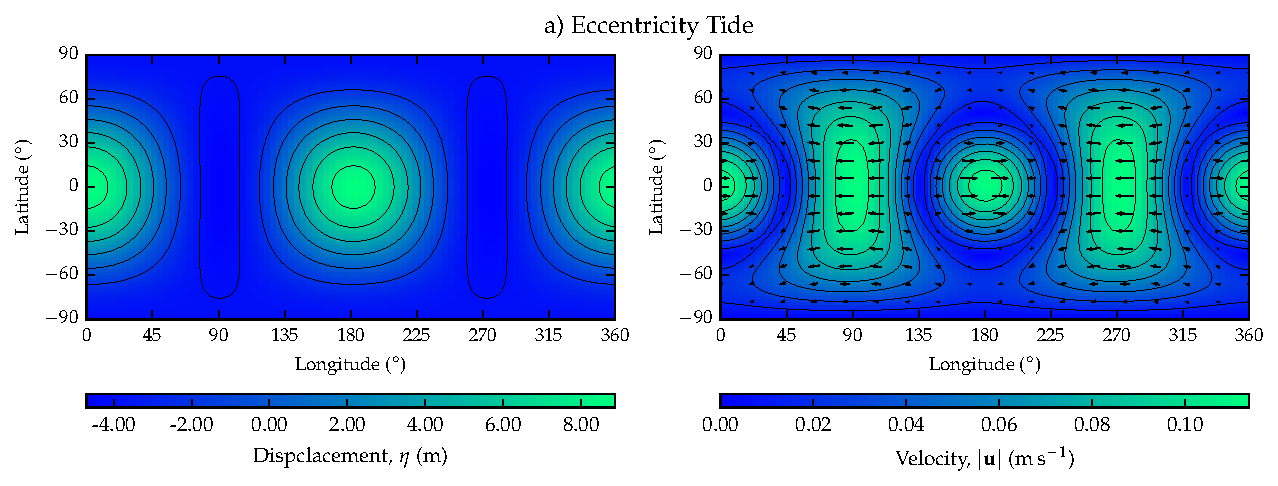
\includegraphics[width=0.8\linewidth,trim={0 0 0 0.2cm},clip]{Figures/Ecc_test}
\subcaption{\label{fig:LTE_a}}
\end{subfigure}\vspace*{-0.7cm}
\begin{subfigure}{\linewidth}
\centering
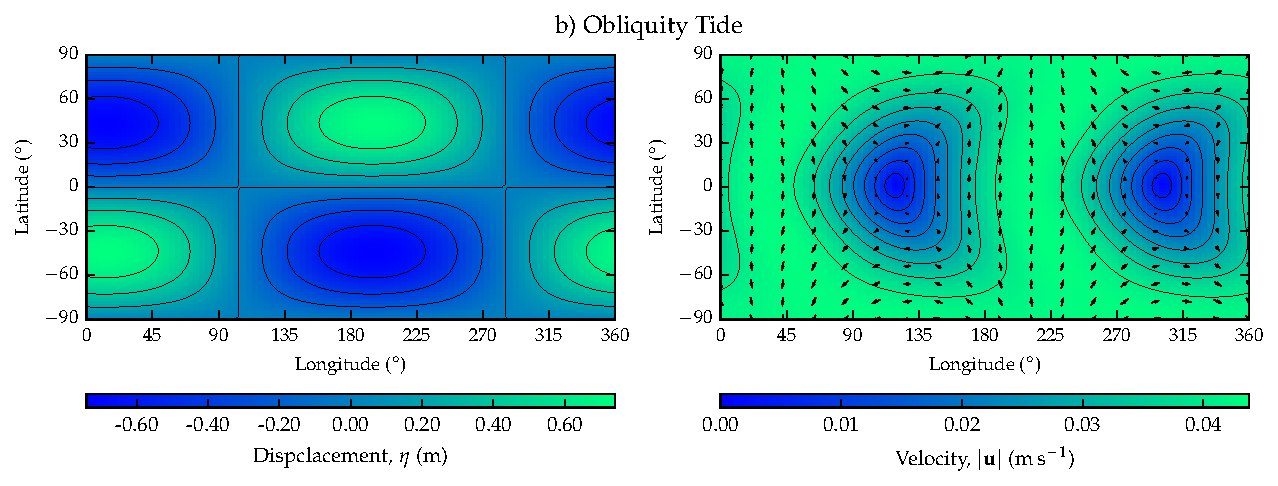
\includegraphics[width=0.8\linewidth]{Figures/Obliq_test}
\subcaption{\label{fig:LTE_b}}
\end{subfigure}\vspace*{-0.7cm}
\begin{subfigure}{\linewidth}
\centering
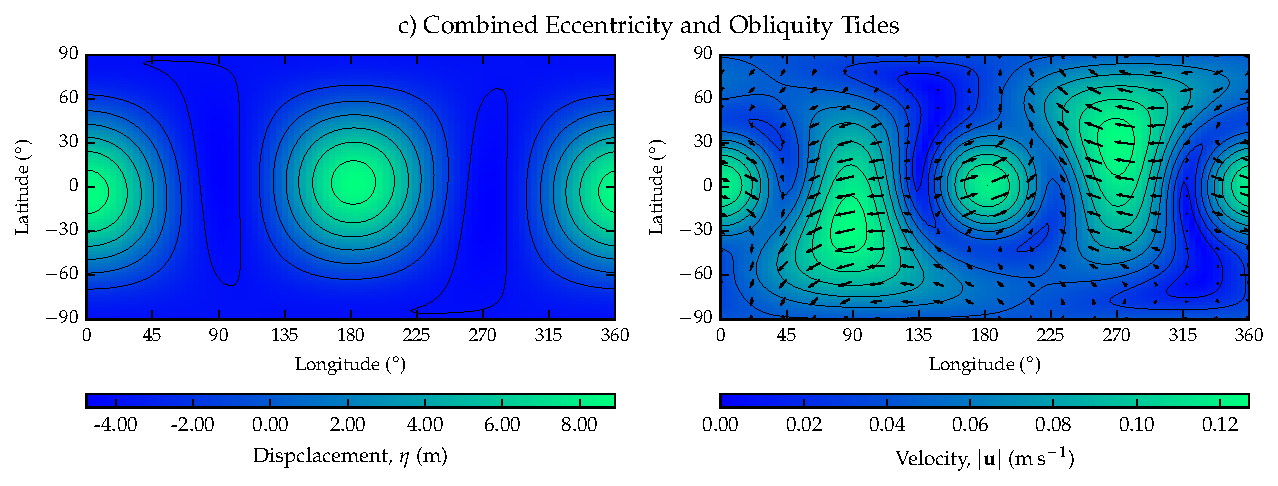
\includegraphics[width=0.8\linewidth]{Figures/Full_test}
\subcaption{\label{fig:LTE_c}}
\end{subfigure}\vspace*{-0.8cm}
\caption{Solutions to the LTE under the eccentricity (eq. \ref{eq:U_ecc}), obliquity (eq. \ref{eq:U_obliq}), and full tidal potential (eq. \ref{eq:U_2}). $h = 400 \, \si{\metre}$ and $\alpha = 2.28 \times 10^{-7} \, \si{\per\second}$ in a), b) and c).\label{fig:LTE_solns}}
\end{figure*}

The primary task of ODIS is to solve the LTE on a sphere, and it is from these solutions that dissipation is derived. Thus, a useful starting point is to illustrate the actual solutions to the LTE rather than purely concerning the reader with the average tidal dissipation over an orbital period. 

Figure \ref{fig:LTE_solns} illustrates numerical solutions to the LTE, at periapse, for different components of the tidal potential on Titan. Surface displacement, $\eta$, is illustrated on the left, whereas velocity, $\bm{u}$, is on the right. The colour scale in the velocity figures represents the velocity's magnitude, $\left| \bm{u} \right|$, Arrows indicate the direction of flow. The tidal forcing applied is, from a) to c), the eccentricity tide, obliquity tide, and both tides combined together, respectively. All plots are for the ``canonical'' $400 \, \si{\metre}$ ocean outlined by \citet{sagan1982tide} to allow best comparison with \citet{sears1994tidal,sears1995tidal,sohl1995tidal}. The coefficient of Rayleigh friction is maintained at $\alpha = 2.28 \times 10^{-7} \, \si{\per\second}$, as mentioned in section \ref{subsec:param}.

Surface displacement in Figure \ref{fig:LTE_a} illustrates a classic tidal bulge, centered on the Saturnian ($\phi = 0^{\circ}$) and sub-Saturian ($\phi = 180^{\circ}$) points. Maximum displacement is over $8$ metres. Away from the tidal bulge displacement drops below the equilibrium level to less than $4$ metres. The corresponding flow pattern shows convergence and divergence at the longitudinal positions of steepest gradient in the displacement field, whereas the fastest flow occurs in the most shallow displacement gradients.

The obliquity tide shows markedly different displacement and flow patterns than the eccentricity tide (Figure \ref{fig:LTE_b}). Displacement is now anti-symmetric about the equator. Notably, the longitudinal positions of maxima and minima are offset from the Saturnian and sub-Saturnian points. The tide raised by the obliquity tidal potential is also an order of magnitude less than the eccentricity tide. Flow is mainly poleward, converging south of the equator on the Saturn-facing hemisphere, and north of the equator on the opposite hemisphere.

The final plot in figure \ref{fig:LTE_solns} is the solution under the full tidal potential. In many ways, it is similar to the eccentricity tide. Yet, the addition of the obliquity tide adds significant equatorial asymmetry to the solutions. This asymmetry is particularly noticeable in the velocity plot on the right hand side of Figure \ref{fig:LTE_c}, where the areas of fastest flow are skewed north and south of the equator, unlike in Figure \ref{fig:LTE_a}. This is also evident in the displacement field, where the tidal bulge maximum does not lie directly on the equator.

\begin{figure}[!t]
\centering
\begin{subfigure}{\linewidth}
\centering
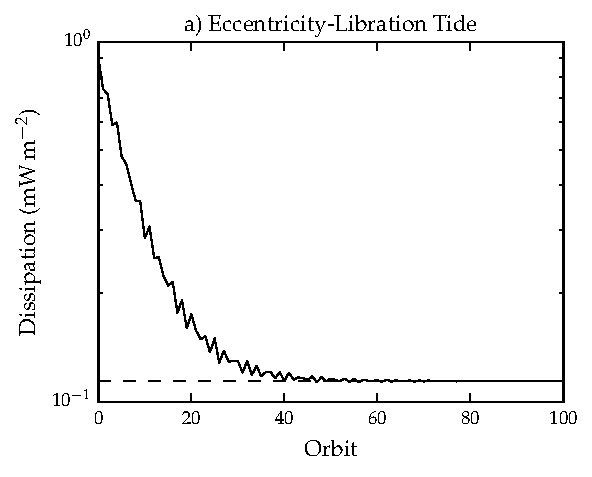
\includegraphics[width=0.8\linewidth]{Figures/ecc_lib_diss}
\subcaption{\label{fig:diss_a}}
\end{subfigure}\vspace*{-0.7cm}
\begin{subfigure}{\linewidth}
\centering
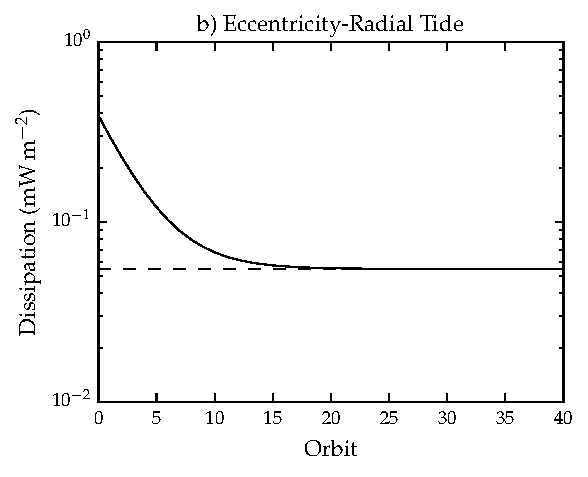
\includegraphics[width=0.8\linewidth]{Figures/ecc_rad_diss}
\subcaption{\label{fig:diss_b}}
\end{subfigure}\vspace*{-0.7cm}
\begin{subfigure}{\linewidth}
\centering
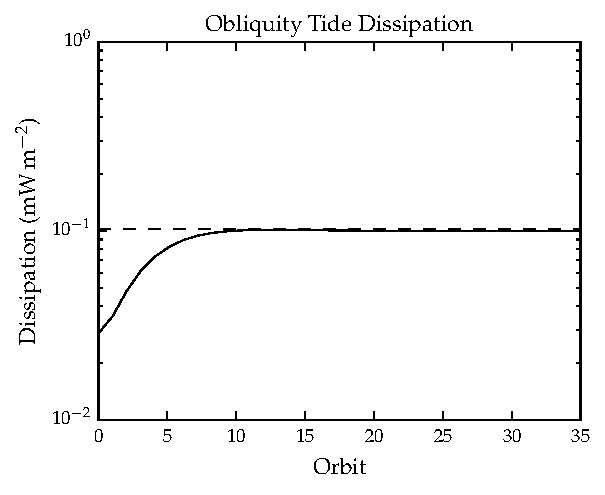
\includegraphics[width=0.8\linewidth]{Figures/obliq_diss}
\subcaption{\label{fig:diss_c}}
\end{subfigure}
\vspace*{-0.8cm}
\caption{Average dissipation over each orbit under the eccentricity-libration, eccentricity-radial, obliquity tides for $h = 400 \, \si{\metre}$ and $\alpha = 2.28 \times 10^{-7} \, \si{\per\second}$ from undisturbed inital conditions on Titan. The dashed lines represent analytical solutions for the time-averaged dissipation. Solid lines are the numerical solution. \label{fig:diss}}
\end{figure}

Comparisons made between the results in Figure \ref{fig:LTE_solns} and the analytical solutions show excellent agreement for this test case.

The simulations used in Figure \ref{fig:LTE_solns} were run from undisturbed initial conditions: \hbox{$\eta = 0 \, \si{\metre}$} and \hbox{$\bm{u} = (0,0) \, \si{\metre\per\second}$}. Consequently, there is some start-up time required for the model to converge into its periodic equilibrium, as described by \citet{sears1995tidal}. Figure \ref{fig:diss} illustrates this issue. From left to right, the figure shows orbitally averaged dissipation against time for the eccentricity-libration, eccentricity-radial, and obliquity tides.  The solid lines represent the average dissipation over each orbit in the numerical model, while the dashed lines indicate the analytical time-averaged dissipation value. 

Initially, the time-averaged dissipation for each model differs from the analytical value. The obliquity tide starts with lower dissipation (fig. \ref{fig:diss_c}), whereas the two components of the eccentricity tide begin with higher dissipation (fig. \ref{fig:diss_a} and \ref{fig:diss_b}). With progressing simulation time, the numerical model then converges onto the analytical value. After 40 Titan orbits, all model values are within $3.5 \si{\percent}$ of the analytical solution. In particular, the eccentricity-radial and obliquity tides are within $1 \si{\percent}$ (Table \ref{tb:diss}). The numerical and analytical time-averaged dissipation values shown in Figure \ref{fig:diss} are given in Table \ref{tb:diss}.

\begin{table}[!b]
\footnotesize
\centering
\begin{tabularx}{\linewidth}{M{2.5cm} M{1.3cm} M{1.3cm} M{1cm}}
 \toprule
Tide & Analytical Dissipation ($\si{\milli\watt\per\metre\squared}$)& ODIS Dissipation ($\si{\milli\watt\per\metre\squared}$) & Error (\%)\\
 \midrule \midrule
Eccentricity-libration & 0.269 & 0.260 & 3.48\\
Eccentricity-radial & 0.0547 & 0.054744 & 0.0802\\
Obliquity & 0.102 & 0.10264 & 0.623\\
\bottomrule
\end{tabularx}
\caption{A comparison of analytical and numerical orbital time-averaged dissipation solutions for $h = 400 \, \si{\metre}$ and $\alpha = 2.28 \times 10^{-7} \, \si{\per\second}$ after 40 Titan orbits. The analytical values are shown as the dashed lines in Figure \ref{fig:diss}. ODIS dissipation values are the final values of the solid lines in Figure \ref{fig:diss}.\label{tb:diss}}
\end{table}

\subsection{Bottom Friction \label{subsec:result_bottom}}

\subsection{Scaling Laws \label{subsec:scaling}}

\section{Discussion \label{sec:discussion}}



\section{Conclusions}

We have designed and implemented a numerical model based on \citet{sears1995tidal} to solve the dissipative Laplace Tidal Equations on a sphere. This model, valid only in the shallow water limit and assuming a global surface ocean, has been used to model ocean flow and its associated tidal dissipation over a range of ocean thicknesses and drag coefficients for both Titan and Enceladus. We neglect the effects of ocean loading and self-attraction.

Modelling is performed with both Rayleigh (linear) and bottom (quadratic) drag models. The former represents internal drag between two adjacent fluid parcels \citep{neumann1968ocean}, while the latter is a global scale approach to incorporating the effects of a macro-scale turbulent boundary layer at some solid-fluid interface \citep{gill1982atmosphere}.

Rayleigh drag results were compared to that of \citet{matsuyama2014tidal} yielding mostly excellent agreement over much of the explored parameter space, providing important validation to our numerical model. Ocean dissipative resonances were replicated well in both Rayleigh and bottom drag simulations. Importantly, we have also demonstrated good agreement between our bottom drag numerical results and the scaling laws of \citet{chen2013tidal} away from gravity-wave resonances, providing further validation of the bottom drag implementation in our model.

For Titan, all gravity-wave resonances occur in very thin oceans and as such  are unlikely to exist. The exception is the Rossby-wave resonance associated with the obliquity tide, which becomes independent of ocean thickness away from thin oceans ($h_0 \leqslant\SI{1}{\kilo\metre}$) in the bottom drag regime. This is also shown in the \citet{chen2013tidal} obliquity tide scaling law. Such a feature means that for a thick ocean on Titan, which is thought to be the case \citep{sohl2014structural}, ocean dissipation becomes dependent on only bottom drag coefficient. For an Earth like bottom drag coefficient we find that ocean dissipation induced by Titan's obliquity tide can reduce its rate of outward orbital migration by  $\sim\SI{40}{\percent}$. Additionally, measurement of $da/dt$ could place constraints on the bottom drag coefficient of Titan's ocean because this resonance becomes independent of ocean thickness. 

Characteristic eccentricity decay times scales for a thick ocean on Titan are found to be well in excess of the age of the Solar System. This is consistent with the relatively high eccentricity observed for Titan at the present day. Any eccentricity damping must therefore come from alternate sources, such as dissipation in the solid regions of the satellite.

Enceladus' eccentricity tide ocean resonances are found to be extremely dissipative, as in \citet{tyler2011tidal, matsuyama2014tidal}. However, the ocean thicknesses where these resonances form are almost certainly too small to be present on Enceladus. We hope to model tidal flow for a spatially varying ocean thickness on Enceladus in the future, as this will likely effect resonant thicknesses and may lead to more localised heating at the SPT. Additionally, it is important to incorporate a solid icy lid into our model to understand how this affects ocean dynamics and dissipation, which will be explored in future work. 

\section*{References}
\bibliography{mybibfile}

\appendix

\section{Laplace Tidal Equations in Spherical Coordinates \label{app:coords}}

To convert the Laplace Tidal Equations to a spherical coordinate system we must make use of the following well-known identities for the gradient and divergence operators,
\begin{equation}
\nabla f = \frac{1}{R} \partial_{\lambda} f \bm{\hat{\lambda}}  
+ \frac{1}{R \cos{\lambda}} \partial_{\lambda} f \bm{\hat{\phi}}
\end{equation}
\begin{equation}
\nabla \cdot \bm{A} = -\frac{1}{R \cos{\lambda}} \partial_{\lambda} \left( \cos{\lambda}\, A_{\lambda} \right) + \frac{1}{R \cos{\lambda}} \partial_{\phi} A_{\phi}
\end{equation}

where $\bm{A}$ is some vector quantity tangent to the spherical surface, $f$ is a scalar quantity, and $\bm{\hat{\lambda}}$ and $\bm{\hat{\phi}}$ are the latitude and longitude unit vectors, also tangent to the surface.
Defining $\bm{u} = \left(u, v \right) = (u_{\phi}, -u_{\lambda} ) $ and using the fact that $\bm{\Omega} = \Omega \bm{\hat{k}}$, where $\bm{\hat{k}}$ is the cartesian unit vector aligned with the rotation axis, then the continuity equation can be rewritten as,
\begin{equation}
\partial_t \eta + \frac{h_0}{R \cos{\lambda}} \left( \partial_{\lambda}
\left(v \cos{\lambda} \right) +  \partial_{\phi} u \right) = 0 \, .
\end{equation}

\noindent Similarly, the momentum equation becomes, 
\begin{equation}
\partial_t u - 2 \Omega v \sin{\lambda}
+ \alpha u
+\frac{c_D}{h_0} \left(u^2 + v^2 \right)^{\nicefrac{1}{2}} u
+ \frac{g}{R \cos{\lambda}} \partial_{\phi} \eta
= 
(1 + k_2 - h_2) \frac{1}{R \cos{\lambda}} \partial_{\phi} U_2
\end{equation}
\begin{equation}
\partial_t v + 2 \Omega u \sin{\lambda}
+ \alpha v
+\frac{c_D}{h_0} \left(u^2 + v^2 \right)^{\nicefrac{1}{2}} v
+ \frac{g}{R} \partial_{\lambda} \eta
= 
(1 + k_2 - h_2) \frac{1}{R} \partial_{\lambda} U_2
\end{equation}

%
%\section{Finite Difference Energy Expressions \}
%
%For a system experiencing both Rayleigh and bottom friction, the full dissipated energy over an orbit is given by,
%\begin{equation}
%F = \frac{\rho}{4 \pi T} \iint \left[h \alpha \left(u^2 + v^2 \right) + c_D \left(u^2 + v^2 \right)^\nicefrac{3}{2} \right}d\Omega dt,
%\end{equation}
%
%\noindent where $\Omega$ is the solid angle and we assume that $h \ll R$.


\end{document}
